
\documentclass[conference,onecolumn]{IEEEtran}
%\documentclass[article,onecolumn]{IEEEtran}
\usepackage{cite}
\usepackage{amsmath,amssymb,amsfonts}
\usepackage{algorithmic}
\usepackage{graphicx}
\usepackage{textcomp}
\usepackage{xcolor}
\usepackage{float}
\usepackage{subcaption}
\usepackage{multirow}
\usepackage{colortbl}
\usepackage{tabularx}
\usepackage{color}
\usepackage{array}
\newcolumntype{P}[1]{>{\centering\arraybackslash}p{#1}}
\definecolor{yellow}{rgb}{0.85, 1,1}
\definecolor{pastleyellow}{rgb}{1, 0.98,0.63}
\setlength{\arrayrulewidth}{0.1mm}
\setlength{\tabcolsep}{6pt}
\setlength\headheight{10pt}


\setlength\parskip{1em plus 0.1em minus 0.2em}
\setlength\parindent{0pt}
\setlength{\parskip}{8pt}
\usepackage{subcaption}
\renewcommand{\arraystretch}{1.5}


\usepackage{tikz}
\usepackage{float}
\usepackage[linesnumbered, ruled,boxed]{algorithm2e}
\usetikzlibrary{trees}
\usetikzlibrary{arrows,shapes,positioning,shadows,trees}

\definecolor{yellow}{rgb}{0.85, 1,1}
\definecolor{pastleyellow}{rgb}{1, 0.98,0.63}
\setlength{\arrayrulewidth}{0.2mm}
\setlength{\tabcolsep}{6pt}
\renewcommand{\arraystretch}{1.5}
\tikzset{
	basic/.style= {draw, text width=2cm, rectangle},
	root/.style = {basic, rounded corners=2pt, thin, align=center},
	level 2/.style = {basic, rounded corners=6pt, thin,align=center,text width=8em},
	level 3/.style = {basic, very thick, rounded corners=3pt, thin,align=center,text width=8em},
	level 4/.style = {basic, thin, align=left, text width=6.5em},
	round/.style = {basic, thin,ellipse}
}


\begin{document}

\title{AUT Report 2023\\}

\author{\IEEEauthorblockN{Akshay Chikhalkar}\\
\IEEEauthorblockA{\textit{Department of Electrical Engineering and Computer Science} \\
\textit{Technische Hochschule Ostwestfalen-Lippe University of Applied Sciences and Arts}\\
Lemgo, Germany \\
akshay.chikhalkar@stud.th-owl.de}

}

\maketitle

\begin{abstract}
This research paper presents a study on the classification of Graphics Processing Units based on graphics memory type. The motivation for this study arose from personal experience as a tech enthusiast, where I recognized the challenge of providing accurate recommendations for technology products in light of the complexity and rapid evolution of the technology domain. The study aims to automate this process by using machine learning algorithms to classify GPUs based on memory type. Three different machine learning algorithms were employed in this study. The performance of these algorithms was evaluated using a confusion matrix and cross-validation. The results of this study demonstrate the effectiveness of using these algorithms for classifying GPUs based on memory type and provide insights into which algorithm is the best fit for this task.\\
\end{abstract}

\begin{IEEEkeywords}
classifier, model, random forest (RFC), decision tree (DTC), support vector machine (SVM), Graphics processing unit (GPU), machine learning (ML)
\end{IEEEkeywords}

\newpage
\tableofcontents

\newpage
\section{Introduction}
\cite{C0}Classification is a powerful technique that allows for faster and more efficient processing of large amounts of data. For technology experts, the ability to quickly and accurately classify data can open up new possibilities for research and experimentation. With the increasing amount of data being generated by devices and applications, the ability to process this data in real-time is becoming increasingly important. GPU classification allows for the creation of more sophisticated models and algorithms, enabling new insights and discoveries. Additionally, the use of GPU classification can significantly reduce the time and resources required for data processing, allowing for more efficient use of resources and cost savings. Overall, GPU classification is a valuable tool for anyone looking to push the boundaries of what is possible with data analysis and machine learning.\\

The current study was motivated by the desire to address the challenge of providing technology recommendations based on multiple factors. I noticed that family members, friends and colleagues often sought advice on technology products, particularly in the realm of computer technology. The complexity of the technology domain, as well as the increasing number of products being released, makes it difficult to keep track of all options and determine the best fit for individual needs.\\

To address this challenge, I proposed a classification solution that utilizes computer processing to classify technology products based on relevant features. The initial focus was the classification of the Graphics Processing Units based on memory type. However, the goal is to not only classify GPUs but also to expand this solution to other technology products.\\

The study aimed to classify GPUs based on memory type, as memory plays a crucial role in the performance of a GPU. Different types of memory, such as DDR3, DDR4, GDDR5 and GDDR6, have different characteristics and can impact the overall performance of a GPU. Three Machine Learning algorithms were employed and the script was written in Python programming language. By classifying GPUs based on memory type, the study aimed to provide a more accurate and comprehensive evaluation of the products available in the market.

\section{Dataset Selection and Description}
\section{Task Solution by State-of-the-Art Classification Methods}

\section{State-of-the-Art Classification Methods}

\subsection{Classification methods}
	In this project, the following classification methods are used to classify the data:

	\subsubsection{Support Vector Machine (SVM)}
	SVM is a supervised learning model with associated learning algorithms that analyze data used for classification and regression analysis. Given a set of training examples, each marked as belonging to one of two categories, an SVM training algorithm builds a model that assigns new examples to one category or the other, making it a non-probabilistic binary linear classifier.
	
	\subsubsection{Random Forest (RF)}
	Random forests or random decision forests are an ensemble learning method for classification, regression and other tasks, that operate by constructing a multitude of decision trees at training time and outputting the class that is the mode of the classes (classification) or mean prediction (regression) of the individual trees. It internally uses decision tree as a base classifier. 
	
	\subsubsection{K-Nearest Neighbors (k-NN)}
	In pattern recognition, the k-nearest neighbors algorithm (k-NN) is a non-parametric method used for classification and regression. In both cases, the input consists of the k closest training examples in the feature space. The output depends on whether k-NN is used for classification or regression. In k-NN classification, the output is a class membership. An object is classified by a majority vote of its neighbors, with the object being assigned to the class most common among its k nearest neighbors (k is a positive integer, typically small). If $k = 1$, then the object is simply assigned to the class of that single nearest neighbor.

	\subsubsection{Gaussian Naive Bayes (GNB)}
	In machine learning, naive Bayes classifiers are a family of simple probabilistic classifiers based on applying Bayes' theorem with strong (naive) independence assumptions between the features. They are among the simplest Bayesian network models. But they could be coupled with Kernel Density Estimation (KDE) to handle continuous data. Naive Bayes has been studied extensively since the 1950s. It was introduced under a different name into the text retrieval community in the early 1960s, and remains a popular (baseline) method for text categorization, the problem of judging documents as belonging to one category or the other (such as spam or legitimate, sports or politics, etc.) with word frequencies as the features. With appropriate pre-processing, it is competitive in this domain with more advanced methods including support vector machines. It also finds application in automatic medical diagnosis.
	
	\subsubsection{Decision Tree Classifier (DTC)}
	Decision tree learning uses a decision tree (as a predictive model) to go from observations about an item (represented in the branches) to conclusions about the item's target value (represented in the leaves). It is one of the predictive modelling approaches used in statistics, data mining and machine learning. Tree models where the target variable can take a discrete set of values are called classification trees; in these tree structures, leaves represent class labels and branches represent conjunctions of features that lead to those class labels. Decision trees where the target variable can take continuous values (typically real numbers) are called regression trees.
	
	\subsubsection{Linear Discriminant Analysis (LDA)}
	In statistics, linear discriminant analysis (LDA), normal discriminant analysis (NDA), or discriminant function analysis is a generalization of Fisher's linear discriminant, a method used in statistics, pattern recognition and machine learning to find a linear combination of features that characterizes or separates two or more classes of objects or events. The resulting combination may be used as a linear classifier, or, more commonly, for dimensionality reduction before later classification.


	\begin{table}[H]
		\centering
		\begin{tabular}{|c|c|c|c|c|c|c|c|}
			\hline
				\textbf{Algorithm} &\textbf{Accuracy} &\textbf{Precision} &\textbf{Recall} &\textbf{F1} &\textbf{E.T. (Sec)} \\ \hline
				\hline
				DTC    & 0.062   & 0.004   & 0.062  & 0.008   & 0.001 \\ \hline
				GNB    & 0.048   & 0.003   & 0.048  & 0.006   & 0.001 \\ \hline
				KNN    & 0.115   & 0.032   & 0.115  & 0.049   & 0.007 \\ \hline
				LDA    & 0.065   & 0.008   & 0.065  & 0.013   & 0.001 \\ \hline
				RFC    & 0.062   & 0.006   & 0.062  & 0.011   & 0.007 \\ \hline
				SVM    & 0.062   & 0.004   & 0.062  & 0.007   & 0.057 \\				
			\hline
		\end{tabular}
		\caption{Classifier performance before dimensionality reduction and hyperparameter optimization}
		\label{tab:performance_before}
	\end{table}




	\begin{figure}[H]
		\centering
		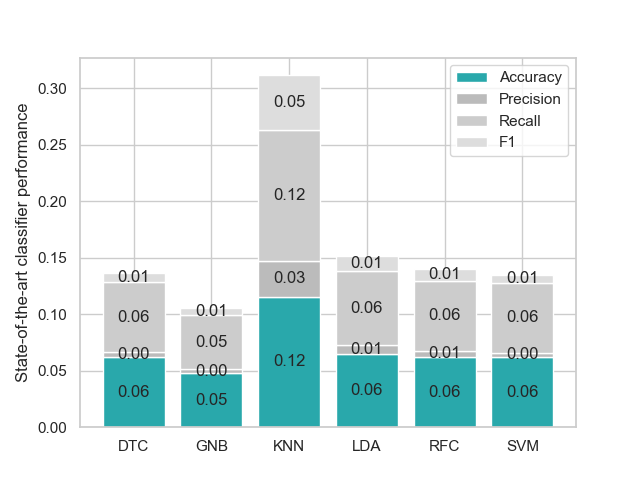
\includegraphics[width=0.5\textwidth]{Plots/Performance_before.png}
		\caption{Classifier performance before dimensionality reduction and hyperparameter optimization}
		\label{fig:performance_before}
	\end{figure}

\subsection{Evaluation methods}
	The evaluation methods used in this project are:
	\subsubsection{Cross-validation}
		Cross-validation is performed using the Stratified K-Fold technique to evaluate the performance of each classifier. Metrics such as \emph{accuracy}, \emph{precision}, \emph{recall} and \emph{F1-score} are calculated and recorded. The results are aggregated and displayed in tabular form, providing insights into the initial accuracy and performance of each classifier. The results are also visualized using a bar chart to provide a more intuitive comparison between the classifiers. 
	\subsubsection{Confusion matrix}
		Confusion matrices are generated to visualize the classification performance of each refined classifier. Heatmap of the correlation matrix for the original features are also created to show correlations among features. 

		The evaluation is performed before and after the feature selection and hyperparameter optimization process to determine the effect of feature selection and hyperparameter optimization on the performance of each classifier. 
	


\section{Increasing Classification Performance: Feature Extraction and Feature Selection}	
\section{Advanced classification methods}
\section{Reduction complexity and execution time}
\section{Conclusion}

% \section{Solutions}
% 	The proposed solution is to use machine learning algorithms to classify Graphics Processing Units based on memory type. This would help to automate the process of product recommendations for technology experts and make it easier to keep track of the ever-demanding technology market. The proposed solution takes advantage of machine learning algorithms such as Random Forest, Decision Tree and Support Vector Machine to classify GPUs based on memory type. The implementation for these algorithm is given below.
% 	\subsection{Classifiers}
% 	\subsubsection[H]{Random Forest}
% 	In 2001, Leo Breiman of the University of California proposed the Random Forest \cite{C26}. It is a classifier composed of a collection of tree-structured classifiers with identically distributed independent random vectors, with each tree casting a unit vote for the most popular class at input $x$\cite{C27}. An upper bound for Random Forests is extracted to get the generalisation error in terms of two parameters exactitude and interdependence of individual classifiers \cite{C25}. \figurename{\ref{Random Forest}} depicts the entire classification process based on the random forest.\\	
% 	\begin{figure}[H]
% 		\centerline{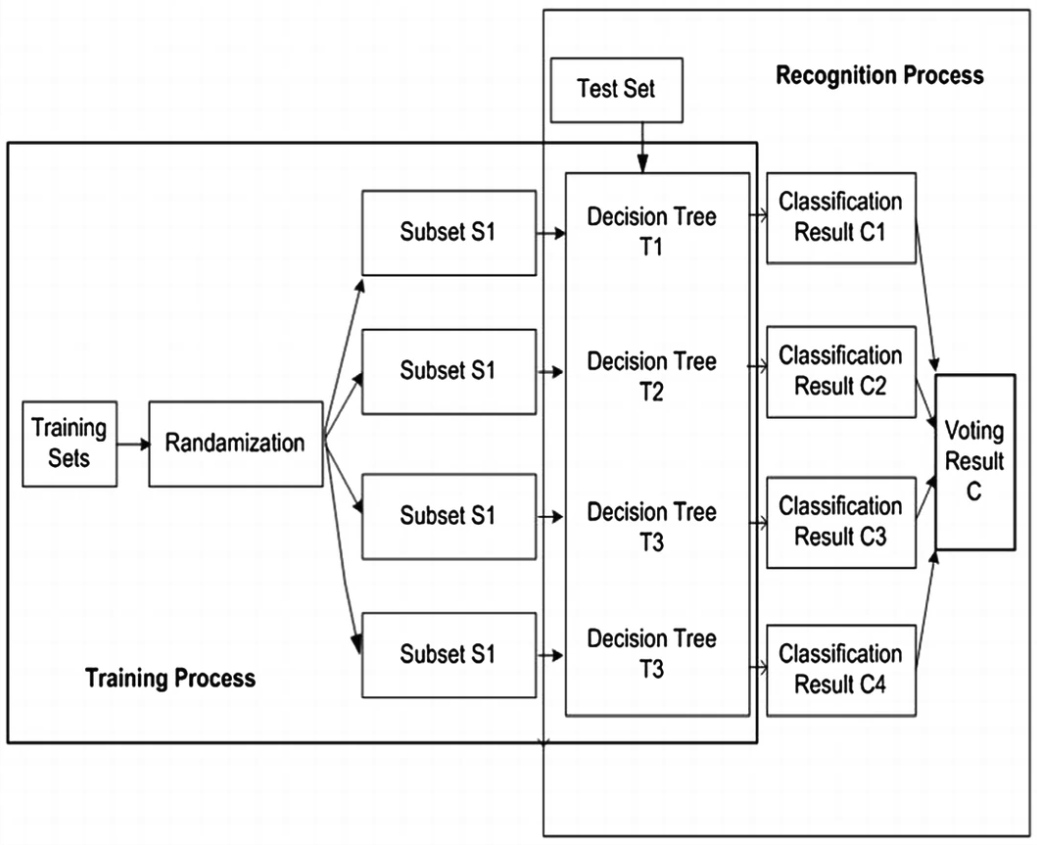
\includegraphics[width=80mm,scale=1]{Images/RandomForest.png}}
% 		\caption{Conceptual framework of random forest classifier\cite{C24}.}
% 		\label{Random Forest}
% 	\end{figure}	
% 	Random forest is a type of ensemble learning algorithm that builds small decision trees with a limited number of features. The random forest categorises data points with each tree and the average of these decision trees becomes the prediction model.\\	
% 	\textbf{Formalization:} The algorithm takes a set of elements as input.\\	
% 	\begin{equation*}
% 			(N,n,e) \to \frac{1}{n} \sum_{i=1}^{n}f_{n}(x,e) \to f(x) \\ 
% 	\end{equation*}
% 	$\text{Where, } N - \text{training data}, e - \text{Entropy}, n - \text{Number of decision trees}$


	

% 	\subsubsection[H]{Decision Tree}		
% 	A decision tree is the most commonly used decision-making tool. To accomplish this, create a decision tree with various branches and leaves. These branches and leaves should represent all of the various aspects of a given situation\cite{C28}. A decision tree functions similarly to a decision support tool. It employs a tree-like graph of decisions and their potential outcomes, such as resource costs, event outcomes and utility. It is one method of displaying an algorithm\cite{C28}. Various types of decision trees can be used depending on the situation and desired outcome.\\	
% 	\begin{figure}[H]
% 		\resizebox{9cm}{!}{
% 			\begin{tikzpicture}[
% 				level 1/.style={sibling distance=32mm},
% 				edge from parent/.style={->,draw},
% 				>=latex]
% 				\node[root] {Decision Node}
% 				child {node[level 2] (c3) {Decision Node}
% 					child {node[round, below=1cm] {Leaf Node}}
% 					child {node[level 3, below=1cm] {Decision Node}
% 						child {node[round] {Leaf Node}}
% 						child {node[round] {Leaf Node}}}}
% 				child {node[level 2] (c2) {Decision Node}
% 					child {node[round, minimum height=1cm] {Leaf Node}}
% 					child {node[round, minimum height=1cm] {Leaf Node}}};				
% 			\end{tikzpicture}
% 		}
% 		\caption[]{Decision tree training flow chart}
% 		\label{Tree Diagram}
% 	\end{figure}
	
% 		A decision tree algorithm is a supervised learning method used for classification and regression problems. The algorithm works by recursively splitting the data into subsets based on the values of input features, creating a tree-like structure. Each internal node of the tree represents a feature and each leaf node represents a class label or a predicted value.
		
% 	    Where, $E$ represents the set of examples, $A$ represents the set of attributes, $PE$ represents the set of parent examples, $T$ represents the decision tree, $A'$ is the most promising attribute and importance(a, E) is a function to find the importance of attribute an over examples E.\\
	
% 	\subsubsection{Support Vector Machine}
	
% 	The C-support vector classification (C-SVC) method is a data mining extension of the SVM (support vector machine) that has many applications in data classification, regression and others\cite{C18}. The letter 'C' in C-SVC stands for the regularisation parameter, which affects the margin of separation between classes. A higher value of C leads to a narrower margin, while a lower value of C leads to a wider margin\cite{C19}.\\
% 	The implementation is built on top of libsvm. Fit time scales at least quadratically with sample number and may be impractical beyond tens of thousands of samples\footnote{https://scikit-learn.org/stable/modules/generated/sklearn.svm.SVC.html}.\\	
% 	Support vector machine is a supervised learning algorithm that determines the decision boundary between two classes of objects. It is a linear or non-linear classifier that distinguishes between the two types of data points. It employs the kernel function to determine a decision boundary between data points for non-linear data points.\\
% 	\textbf{Formalization:} The algorithm take a set of an element as input.\\	
% 	\begin{equation*}
% 		(N, K) \rightarrow \sum_{i=1}^{n} \alpha_{i} \ \ y_{i} \ \ K(x_{i}, x) + b \rightarrow f(x)
% 	\end{equation*}
% 		Where, $N-$ training data, $K-$ kernel function
% 	\begin{algorithm}[!ht]
% 		\vspace{1em}
% 		\KwIn{\small Data set \( N \)}
% 		\KwOut{\small Find differnent classes of objects}
		
% 		\vspace{1em}
		
% 		\SetKwFunction{FMain}{SVC}
% 		\SetKwProg{Fn}{Function}{:}{}
% 		\Fn{\FMain{$X$, $y$, $k$}}
% 		{
% 			$V \leftarrow \phi$\;
% 			\For{$x \in X$}
% 			{
% 				$x_{k} = k(X);$\\
% 				$v= v - x_{k};$\\
% 				$V \leftarrow V \cup v;$\\
% 			}
% 			\Return{\( V ;\)}
% 		}
% 		\label{Support Vector Machine}
% 		\vspace{1em}
% 		\caption{Support vector machine}%
% 	\end{algorithm}

% 	\subsubsection{Performance Metrics}
% 	A Confusion Matrix and Cross-Validation are both commonly used performance matrices for evaluating the effectiveness of classification algorithms in ML.
	
% 	\textit{Confusion matrix:}
% 	A Confusion Matrix is a commonly used performance matrix for classification algorithms. It is a table that is used to compare the predicted values of a model with the actual values and it is particularly useful for classification problems with multiple output classes. The matrix is organized as an N*N table, where N represents the number of output classes. The four different combinations of predicted and actual values are represented in the matrix and are used to calculate other performance metrics such as accuracy, precision, recall and F1-score\cite{C34}.
	
% 	The Confusion matrix typically contains the following four combinations of predicted and actual values:
% 	\begin{itemize}
% 	\item True Positives (TP) - the number of observations that are correctly predicted as positive
% 	\item False Positives (FP) - the number of observations that are incorrectly predicted as positive
% 	\item True Negatives (TN) - the number of observations that are correctly predicted as negative
% 	\item False Negatives (FN) - the number of observations that are incorrectly predicted as negative
% 	\end{itemize}

% 	These values are used to calculate various metrics such as accuracy, precision, recall and F1-score which gives a holistic view of the performance of the model\cite{C35}.
	
% 	\noindent Accuracy is defined as the ratio of correctly predicted observations to total observations\cite{C35}.
% 	\begin{equation*}
% 		Accuracy = \frac{(TP + TN)} {(TP + FP +TN + FN)}
% 	\end{equation*}
	
% 	\noindent Precision is defined as the ratio of true positive values to total correctly predicted values \cite{C35}.
% 	\begin{equation*}
% Precision = \frac{TP}{(TP + FP)}
% 	\end{equation*}
	
% 	\noindent The number of correctly predicted values from all positive classes is defined as recall. It is also known as sensitivity\cite{C36}.
	
% 	\begin{equation*}
% 		Recall = \frac{TP}{(TP + FP)}
% 	\end{equation*}
	
% 	\noindent The F\textsubscript{1} score is the weighted average of precision \& recall\footnote{https://en.wikipedia.org/wiki/F-score}.
	
% 	\begin{equation*}
% 		{\displaystyle F_{1}=2{\frac {\mathrm {precision} \cdot \mathrm {recall} }{\mathrm {precision} +\mathrm {recall} }}={\frac {2\mathrm {tp} }{2\mathrm {tp} +\mathrm {fp} +\mathrm {fn} }}}
% 	\end{equation*}
% 	\\
% 	\textit{Cross-validation - StratifiedKFold:}
% 	Cross-validation is a technique that is used to assess the performance of a model by splitting the data into several partitions, training the model on one partition and testing it on the other partition\cite{C37}. This is done multiple times, each time using a different partition for testing and the results are then averaged to give an overall estimate of the model's performance\cite{C37}.
% 	StratifiedKFold is a variation of K-fold cross-validation that ensures each fold has a similar proportion of samples from each class. It was used with 10 folds for better cross-validation and tested 1200+ times to account for variations in execution time.
% \section{Experiments and Results}
% 	\noindent \textit{Data Preparation}: A Kaggle dataset named Data Mining UNDIP\footnote{https://www.kaggle.com/code/yukihm/data-mining-undip} was chosen for this classification simulation. It contained a total of  \textbf{2889} samples and \textbf{16} feature, out of which \textbf{5} features were considered to train the models (Dependent Variable - Memory Type and Independent Variables - Memory Size, GPU Clock, Memory Clock, Memory Bus Width), refer to \figurename{\ref{dataset}}. Interpolation was used for generating and filling in missing values in the dataset. The dataset was split into \textbf{80-20\%} for training and testing respectively.
% 	\begin{figure}[H]{}
% 	\centerline{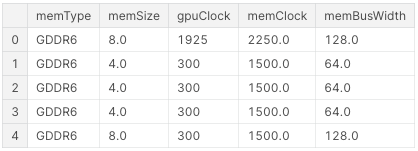
\includegraphics[width=90mm,scale=1]{Images/dataset.png}}
% 	\caption{Dataset snapshot}
% 	\label{dataset}
% 	\end{figure}
% 	A pearson's correlation was performed to check the correlation between independent variables. It resulted in correlation between all four features which can be verified from the correlation heatmap, refer to \figurename{\ref{DataCorelation}}. For further dataset analysis and visualisation, refer to Appendix \figurename{\ref{DataBarplot}}, \figurename{\ref{DatagpuClockvsmemClock}} and \figurename{\ref{DataPariPlot}}.
% 		\begin{figure}[H]
% 		\centerline{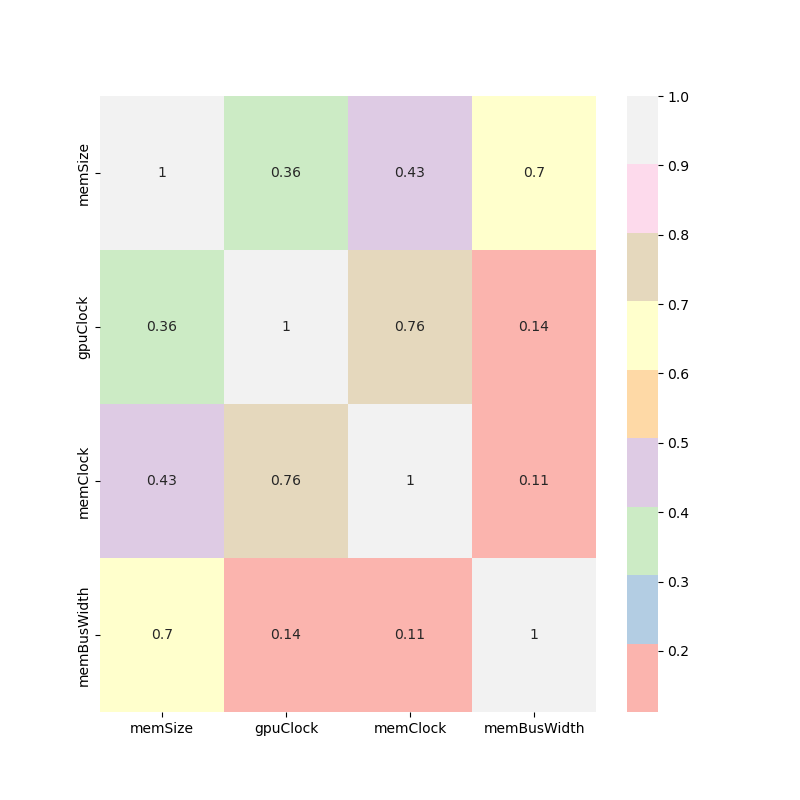
\includegraphics[width=95mm,scale=1]{Images/DataCorelation.png}}
% 		\caption{Data correlation heatmap}
% 		\label{DataCorelation}
% 	\end{figure}
% 	\noindent \textit{Algorithm Selection}: Three different machine learning algorithms were employed in this study: Random Forest, Decision Tree and Support Vector Machine. These algorithms were chosen as they have been widely used in similar classification tasks and have been shown to produce accurate results.
% 	\textit{Algorithm Training}: Each algorithm was trained using the selected features from the dataset and the trained models were used to classify the GPUs based on the memory type.
% 	\textit{Evaluation}: The performance for three classifiers (Random Forest, Decision Tree and Support Vector Machine) was evaluated using two techniques, Confusion Matrix and Cross-validation. In cross-validation, along with accuracy, execution time was recorded for over 1200 tests.
% 	\textit{Note 1}: The performance evaluation for all three algorithms was measured without parameter optimisation.\\
% 	\textit{Note 2}: The entire benchmarking was performed using macOS Ventura 13.1 (22C65) running on Apple Macbook Air, Apple M1 (8-Core CPU) and LPDDR4X 16GB RAM.
% 	\subsection{Confusion matrix results}
% 	In the Confusion Matrix performance evaluation, Accuracy, Precision, Recall and F1 score were recorded on a scale of 0 to 1 (0 being worst and 1 being best). For confusion matrix heatmap plot for all three calssifiers, refer to Appendix \figurename\ref{Confussion matrix heatmap}.
% 		\begin{figure}[H]{}
% 		\centerline{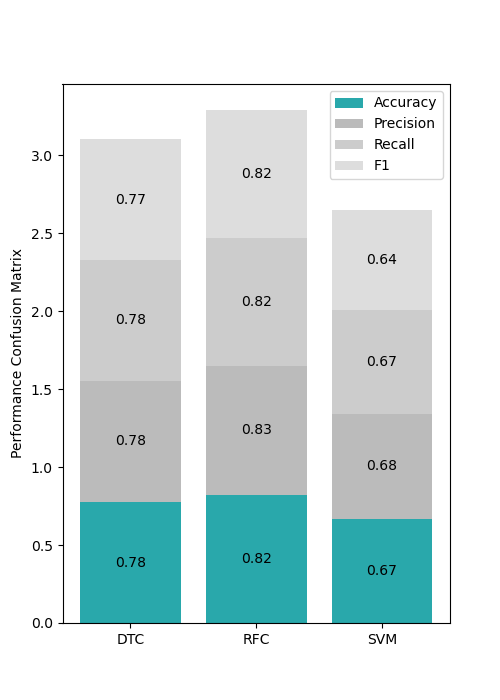
\includegraphics[width=80mm,scale=1]{Images/Performance_CM.png}}
% 		\caption{Performance based on confusion matrix results}
% 		\label{Performance_CM}
% 	\end{figure}
% 	RFC outperforms other classifiers (DTC and SVM) in each aspect. It has the highest sectional and overall score, refer to \figurename{\ref{Performance_CM}}. However, DTC perform second best and SVM was last.\\
% 	Clearly from the performance wise Random Forest comes out as the best classification algorithm in comparison with Decision Tree and Support Vector Machine. Refer to \figurename{\ref{Performance_CM}} for confusion matrix results.\\
% 	Based on these results, it appears that the Random Forest Classifier has the highest accuracy, precision, recall and F1-score among the three algorithms. The Decision Tree Classifier also performed well in terms of accuracy, precision and recall while SVM performed proorly.
%  \subsection{Cross-validation results}

% 		\begin{figure}[H]% ! doesn't do what you think it does
% 			\centering
% 			\begin{subfigure}[t]{4cm}
% 				\centerline{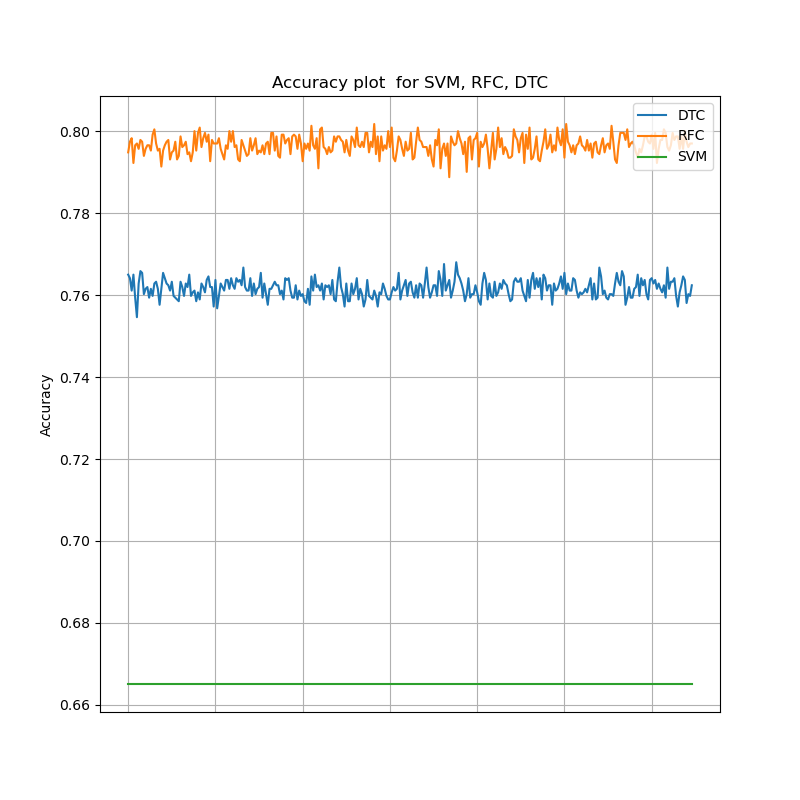
\includegraphics[width=4.7cm,scale=1]{Images/Accuracy Plot.png}}
% 				\caption{Accuracy plot}
% 				\label{Accuracy Plot}
% 			\end{subfigure}\hfil% equal to outside spacing
% 			\begin{subfigure}[t]{4cm}
% 				\centerline{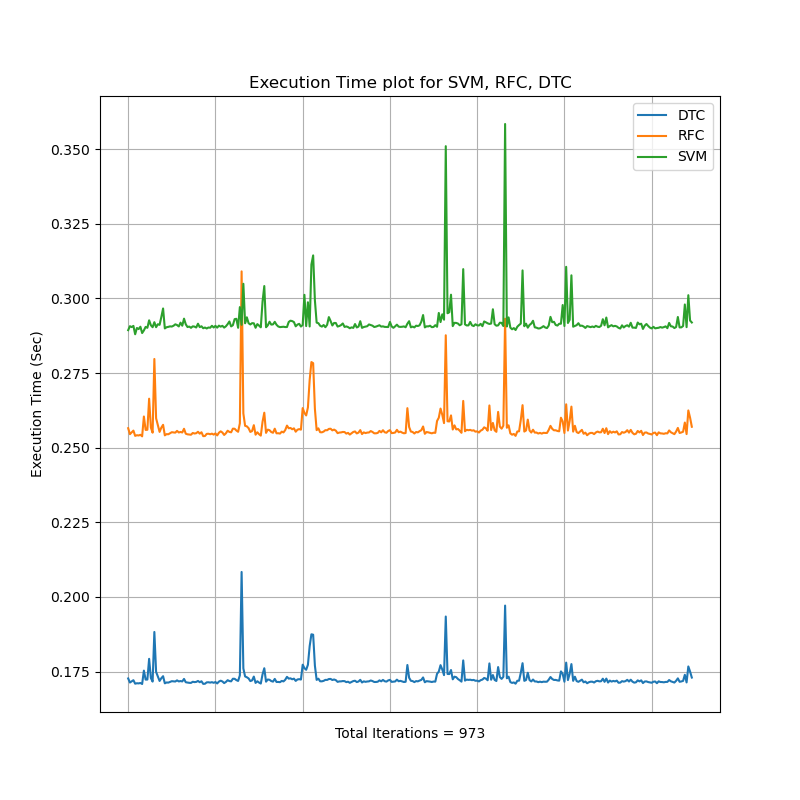
\includegraphics[width=4.7cm,scale=1]{Images/Execution Time Plot.png}}
% 				\caption{Execution time plot}
% 				\label{Execution Time Plot}
% 			\end{subfigure}
% 		\caption{Accuracy and execution time plot}
% 		\label{Accuracy and Execution Time Plot}
% 		\end{figure}	
% 	\begin{figure}[H]
% 	\centerline{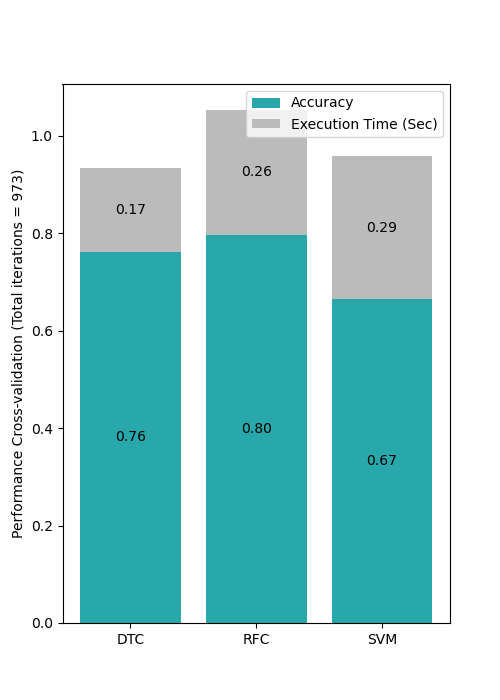
\includegraphics[width=80mm,scale=1]{Images/Performance_CV.png}}
% 	\caption{Performance based on cross-validation results}
% 	\label{Performance_CV}
% 	\end{figure}	
% 	In terms of execution time, DTC outperformed RFC and SVM by taking the lowest time with \textbf{0.17 Sec}. RFC and SVM performed approximately the same with a of \textbf{0.03 }second difference between them.
% 	To see the variations in accuracy and execution time for over 1200 tests, refer to \figurename{\ref{Accuracy and Execution Time Plot}}
% 	Note: The average was taken from 1261 test results for each classifier.
% 	All three algorithms (DTC, RFC and SVM) showed consistent performance after over 1200 cross-validation tests. SVM was particularly stable with an accuracy of \textbf{0.66}. DTC's accuracy varied between \textbf{0.75} and \textbf{0.77}, while RFC's accuracy ranged from \textbf{0.79} to \textbf{0.81}. Refer to \figurename{\ref{Performance_CV}} for cross-validation results.
% %	\begin{table}[H]	
% %	\begin{center}
% %	\begin{tabular}{|c|c|c|c|}
% %		\hline
% %		\textbf{Classifier Name}&\textbf{Accuracy}  &\textbf{Execution Time} &\textbf{Iterations}   \\ \hline
% %		DTC          &0.761        &0.241     &183     \\ \hline
% %		RFC          &0.796        &0.358     &183	\\ \hline
% %		SVM        	&0.665       &0.366  	 &183     \\ 
% %		\hline
% %	\end{tabular}
% %	\end{center}
% %	\caption{Cross-validation results}
% %	\label{Results_CV}
% %	\end{table}
% 	\begin{table}[H]	
% 		\begin{center}
% 			\begin{tabular}[H]{ |p{1.5cm}|p{1.5cm}|p{1.5cm}|p{0.7cm}|p{0.7cm}|p{0.7cm}|p{1.5cm}|}
% 				\hline
% 				\multicolumn{7}{|c|}{\textbf{Combined Results}} \\
% 				\hline
% 				\textbf{Classifier}&\textbf{Accu. (CV)} &\textbf{Accu. (CM)} &\textbf{P} &\textbf{R}  &\textbf{F}$_{1}$ &\textbf{ET (sec)}  \\ \hline
% 				DTC 	&0.761 &0.776 &0.779 &0.776 &0.775 &0.171  \\ \hline
% 				\rowcolor{pastleyellow} RFC 	&0.796 &0.820 &0.821 &0.820 &0.819 &0.255  \\ \hline
% 				SVM 	&0.665 &0.666 &0.676 &0.666 &0.639 &0.287   \\ 
% 				\hline
% 			\end{tabular}
% 		\end{center}
% 		\caption{Overall results}
% 		\label{Overall Results}
% 	\end{table}
% 	The results of the study indicate that the Random Forest Classifier performed the best among the three algorithms considered in this study. The Random Forest Classifier achieved the highest score of \textbf{0.82} in cross-validation (CV) and also had the highest accuracy (Accu.), precision (P), recall (R) and F1-score among the three algorithms as per confusion matrix (CM). Additionally, the Decision Tree Classifier also performed well in terms of accuracy, precision and recall but Random Forest Classifier performed better than DTC. However, the Support Vector Machine had the lowest performance among the three algorithms in all the evaluation metrics. The execution time (ET) for the Random Forest classifier is slightly higher than the Decision Tree Classifier, while Support Vector Machine has the highest execution time among the three classifiers, refer to \figurename{\ref{Overall Results}}.
% \section{Summary and Outlook}
	The results of the study showed that the Random Forest algorithm had the highest accuracy in classifying the GPU based on memory type, followed by Decision Tree and Support Vector Machine. The study also evaluated the performance of the algorithms based on precision, recall and F1-score, which are commonly used metrics for evaluating the performance of classification models. However, it should be noted that the study did not include any parameter optimization and the performance could potentially be improved through hypermeter tuning.
	
	The study concludes that the proposed classification solution, which utilizes computer processing and machine learning algorithms, can effectively classify GPUs based on memory type. The results of this study can be used to provide more accurate recommendations for technology products and can be extended to other technology products as well. This research can be used as a foundation for further research in the field of technology product classification and it can be useful for consumers, manufacturers and retailers. 
	

\newpage
\section*{Appendix}

    \begin{table}[H]	
        \begin{center}
            \begin{tabular}[H]{ |m{1cm}|m{1cm}|m{1.2cm}|m{1.2cm}|m{1cm}|m{2cm}|m{3cm}|m{2cm}|}
                \hline
                \textbf{Item}&\textbf{Mean} &\textbf{Variance} &\textbf{Std. Dev.}  &\textbf{No.}  &\textbf{Left} &\textbf{Right} &\textbf{Scale}\\ \hline
                1	&1,8	&0,2	&0,4	&5	&annoying	            &enjoyable	                &Attractiveness             \\ \hline
                2	&2,2	&0,2	&0,4	&5	&not                    &understandable	            &understandable         \\ \hline
                3	&0,6	&2,3	&1,5	&5	&creative	            &dull	                    &Novelty        \\ \hline
                4	&3,0	&0,0	&0,0	&5	&easy to learn	        &difficult to learn	        &Perspicuity        \\ \hline
                5	&2,2	&0,2	&0,4	&5	&valuable	            &inferior	                &Stimulation        \\ \hline
                6	&0,8	&1,7	&1,3	&5	&boring	                &exciting	                &Stimulation        \\ \hline
                7	&1,8	&0,7	&0,8	&5	&not interesting	    &interesting	            &Stimulation        \\ \hline
                8	&2,2	&1,2	&1,1	&5	&unpredictable	        &predictable	            &Dependability      \\ \hline
                9	&2,2	&1,7	&1,3	&5	&fast	                &slow	                    &Efficiency     \\ \hline
                10	&-1,4	&2,3	&1,5	&5	&inventive	            &conventional	            &Novelty        \\ \hline
                11	&2,4	&0,3	&0,5	&5	&obstructive	        &supportive	                &Dependability      \\ \hline
                12	&2,2	&0,7	&0,8	&5	&good	                &bad	                    &Attractiveness     \\ \hline
                13	&1,2	&5,7	&2,4	&5	&complicated	        &easy	                    &Perspicuity        \\ \hline
                14	&2,0	&1,0	&1,0	&5	&unlikable	            &pleasing	                &Attractiveness     \\ \hline
                15	&-1,2	&2,7	&1,6	&5	&usual	                &leading edge	            &Novelty        \\ \hline
                16	&2,0	&0,5	&0,7	&5	&unpleasant	            &pleasant	                &Attractiveness     \\ \hline
                17	&2,4	&0,8	&0,9	&5	&secure	                &not secure	                &Dependability      \\ \hline
                18	&1,8	&0,2	&0,4	&5	&motivating	            &demotivating	            &Stimulation        \\ \hline
                19	&2,2	&1,7	&1,3	&5	&meets			        &does not meet				&Dependability      \\ \hline
                20	&2,6	&0,3	&0,5	&5	&inefficient	        &efficient	                &Efficiency     \\ \hline
                21	&1,8	&0,7	&0,8	&5	&clear	                &confusing	                &Perspicuity        \\ \hline
                22	&2,2	&0,7	&0,8	&5	&impractical	        &practical	                &Efficiency     \\ \hline
                23	&2,0	&1,0	&1,0	&5	&organized	            &cluttered	                &Efficiency     \\ \hline
                24	&2,0	&1,5	&1,2	&5	&attractive	            &unattractive	            &Attractiveness     \\ \hline
                25	&2,2	&0,7	&0,8	&5	&friendly	            &unfriendly	                &Attractiveness     \\ \hline
                26	&-1,4	&2,3	&1,5	&5	&conservative	        &innovative	                &Novelty        \\ 
                \hline
            \end{tabular}
        \end{center}
        \caption{Mean value per item}
        \label{table:Mean value per item}
    \end{table}


\newpage
\bibliographystyle{IEEEtran}
\bibliography{ref}
\end{document}